\section{Experimental Evaluation}
\label{sec:experiments}
    \begin{figure*}[t]
		\centering
		\begin{subfigure}[t]{0.24\linewidth}
			\centering
			\includegraphics[width = \linewidth]{./img/sine6.pdf}
		\end{subfigure}
		\begin{subfigure}[t]{0.24\linewidth}
			\centering
			\includegraphics[width = \linewidth]{./img/sine14.pdf}
		\end{subfigure}
		\begin{subfigure}[t]{0.24\linewidth}
			\centering
			\includegraphics[width = \linewidth]{./img/line5.pdf}
		\end{subfigure}
		\begin{subfigure}[t]{0.24\linewidth}
			\centering
			\includegraphics[width = \linewidth]{./img/line16.pdf}
		\end{subfigure}
		\\
		\includegraphics[height=1.5em]{./img/legend_mixed_maml.pdf}
		\caption{SImPa and MAML are compared in a regression problem when training is based on multi-modal data -- half of the tasks are generated from sinusoidal functions, and the other half are from linear functions. The shaded area is the prediction made by SImPa \(\pm\) 3\(\times\) standard deviation.}
		\label{fig:regression_visualisation}
	\end{figure*}
        
        \begin{figure*}[t]
        	\centering
\begin{subfigure}[b]{0.25 \linewidth}
        	    \centering
\begin{tikzpicture}
                    \pgfplotstableread[col sep=&, row sep=\\, header=true]{
                        method & nll\\
                        MAML & 2.32\\
                        PLATIPUS & 2.52\\
                        BMAML & 1.45\\
                        ABML & 2.65\\
                        SImPa & 1.58\\
                    } \myTable

                    \pgfplotstablegetrowsof{\myTable}
                    \pgfmathsetmacro{\NumRows}{\pgfplotsretval-1}

                    \begin{axis}[
                        height = 0.9 \linewidth,
                        width = 0.9 \linewidth,
                        xbar = 0pt,
                        xmin = 1.25,
                        xmax = 2.75,
                        xticklabel style = {font=\footnotesize},
                        xlabel={Mean squared error},
                        xlabel style = {font=\footnotesize},
                        ytick=data,
                        yticklabels from table={\myTable}{method},
                        yticklabel style = {font=\footnotesize, align=left},scale only axis,
                        enlarge x limits=auto,
                        enlarge y limits=0.1,
                        grid=major,
                        grid style={dotted, thick},
                        every axis plot/.append style={fill=NavyBlue, draw=none}
                    ]
                        \addplot[] table [y expr=\NumRows - \coordindex, x=nll]{\myTable};
                    \end{axis}
                \end{tikzpicture}
        	    \caption{MSE on hold-out tasks}
        	    \label{fig:SImPa_regression_NLL}
        	\end{subfigure}
        	\hspace{2em}
        	\hfill
        	\begin{subfigure}[b]{0.25\linewidth}
        		\centering
                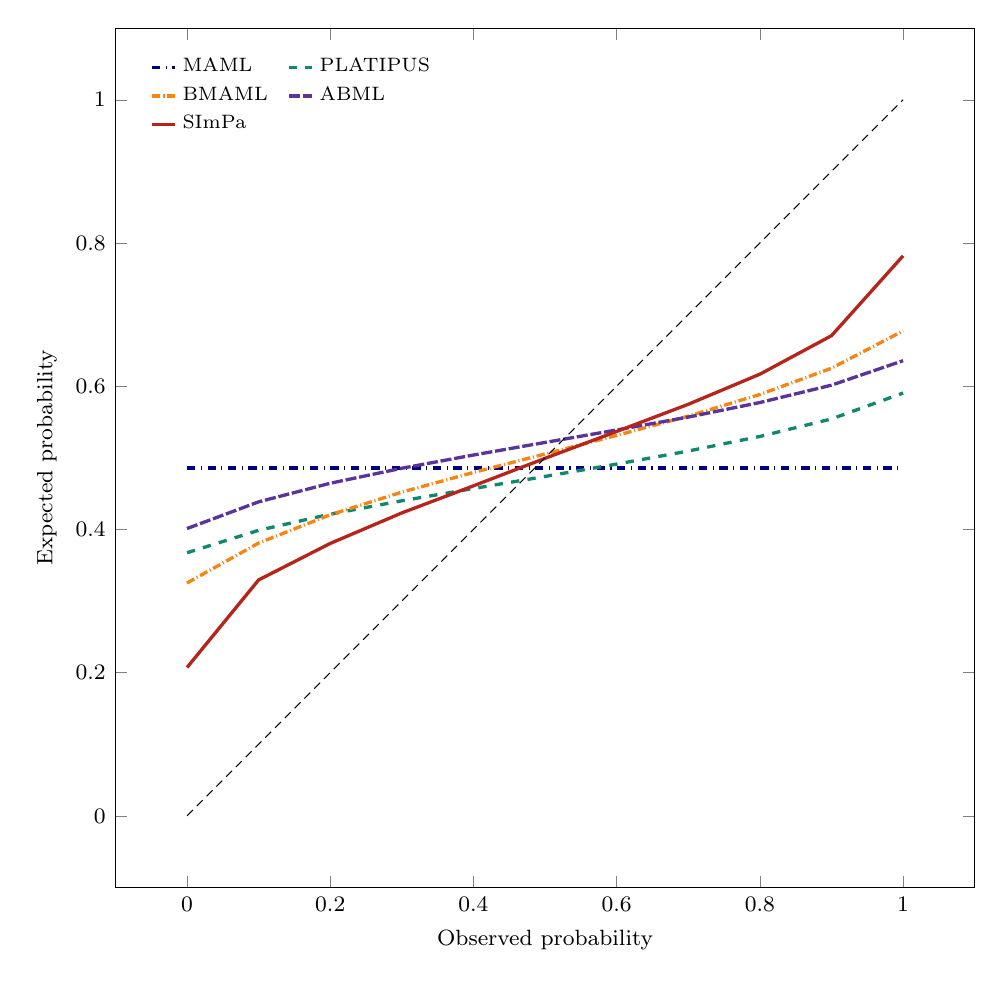
\begin{tikzpicture}
                    \pgfplotstableread[col sep=comma, row sep=\\, header=true]{
                        x,MAML,PLATIPUS,BMAML,ABML,SImPa\\
                        0,0.4860619902610778809,0.36753817,0.32526379,0.40130252,0.20724078\\
                        0.1,0.4860619902610778809,0.39879262,0.38103479,0.43856199,0.32954753\\
                        0.2,0.4860619902610778809,0.42135352,0.42053903,0.464544,0.3804987\\
                        0.3,0.4860619902610778809,0.44004638,0.45217654,0.48548708,0.42313374\\
                        0.4,0.4860619902610778809,0.4571563,0.47961517,0.50396608,0.46094437\\
                        0.5,0.4860619902610778809,0.47404441,0.50541934,0.52153283,0.49935024\\
                        0.6,0.4860619902610778809,0.49129097,0.53134508,0.53895331,0.53686566\\
                        0.7,0.4860619902610778809,0.50953219,0.55830806,0.55695198,0.57479658\\
                        0.8,0.4860619902610778809,0.52991487,0.58850907,0.57726778,0.61686458\\
                        0.9,0.4860619902610778809,0.55434502,0.62519009,0.60150843,0.67059377\\
                        1,0.4860619902610778809,0.59050844,0.67733319,0.63569099,0.78212945\\
                    } \calibrationTable
                    
                    \begin{axis}[
                        height = 0.9 \linewidth,
                        width = 0.9 \linewidth,
                        xlabel={Observed probability},
                        xlabel style={font=\footnotesize},
                        xticklabel style = {font=\footnotesize},
                        ylabel={Expected probability},
                        ylabel style = {font=\footnotesize, yshift=0em},
                        yticklabel style = {font=\footnotesize},
scale only axis,
                        table/x=x,
                        legend entries = {MAML, PLATIPUS, BMAML, ABML, SImPa},
                        legend style = {draw=none, font=\scriptsize, yshift=0.25em, /tikz/every even column/.append style={column sep=0.5em}},
                        legend cell align = {left},
                        legend columns = 2,
                        legend image post style={scale=0.5},
                        legend pos = north west
                    ]
                        \addplot[mark=none, NavyBlue, dashdotted, very thick] table[y={MAML}]{\calibrationTable};
                        \addplot[mark=none, PineGreen, dashed, very thick] table[y= {PLATIPUS}]{\calibrationTable};
                        \addplot[mark=none, BurntOrange, densely dashdotted, very thick] table[y = {BMAML}]{\calibrationTable};
                        \addplot[mark=none, RoyalPurple, dash pattern=on 4pt off 1pt, very thick] table[y = {ABML}]{\calibrationTable};
                        \addplot[mark=none, BrickRed, solid, very thick] table[y = {SImPa}]{\calibrationTable};
                        
                        \addplot[mark=none, Black, densely dashed] table[y = {x}]{\calibrationTable};
                    \end{axis}
                \end{tikzpicture}
        		\caption{Reliability diagram}
        		\label{fig:SImPa_regression_reliability_chart}
        	\end{subfigure}
        	\hfill
        	\begin{subfigure}[b]{0.25\linewidth}
\begin{tikzpicture}
                    \pgfplotstableread[col sep=comma, row sep=\\, header=true]{
                        method,ECE,MCE\\
                        MAML,0.2739943645217202,0.5139380097389221\\
                        PLATIPUS,0.2213864627272727,0.40949156\\
                        BMAML,0.18939665181818183,0.32526379\\
                        ABML,0.21863836454545452,0.40130252\\
                        SImPa,0.14734225818181818,0.22954752999999997\\
                    } \ceTable
                    
                    \pgfplotstablegetrowsof{\ceTable}
                    \pgfmathsetmacro{\NumRows}{\pgfplotsretval-1}

                    \begin{axis}[
                        width = 0.9 \linewidth,
                        height = 0.9 \linewidth,
                        xbar=0pt,
                        ytick=data,
                        yticklabels from table={\ceTable}{method},
                        yticklabel style = {font=\footnotesize},
                        xticklabel style = {font=\footnotesize},
                        xlabel style = {font=\footnotesize},
                        xlabel = {Calibration error},
                        scale only axis,
enlarge x limits=auto,
                        enlarge y limits=0.15,
                        grid=major,
                        grid style={dotted, thick},
                        every axis plot/.append style={fill, draw=none},
                        legend entries = {ECE,MCE},
                        legend style = {draw=none, font=\scriptsize, yshift=0em, /tikz/every even column/.append style={column sep=0.5em}},
                        legend cell align = {left},
                        legend columns = 2,
                        legend image post style={scale=1},
                        legend pos = south east
                    ]
                        \addplot[mark=none, NavyBlue] table [y expr=\NumRows - \coordindex, x = {ECE}] {\ceTable};
                        \addplot[mark=none, BrickRed] table [y expr=\NumRows - \coordindex, x = {MCE}] {\ceTable};
                    \end{axis}
                \end{tikzpicture}
        		\caption{ECE and MCE}
        		\label{fig:SImPa_regression_ECE_MCE}
        	\end{subfigure}
        	\hfill
        	\hphantom{x}

        	\caption{Quantitative comparison between various probabilistic meta-learning approaches averaged over 1000 unseen tasks shows that SImPa has a comparable MSE error and the smallest calibration error.}
        	\label{fig:regression_calibration}
        \end{figure*}

    In this section, SImPa is evaluated on few-shot regression and classification problems and compared to common meta-learning baselines, such as MAML~\citep{finn2017model}, ABML~\citep{ravi2018amortized}, PLATIPUS~\citep{finn2018probabilistic} and BMAML~\citep{yoon2018bayesian}.

    In the experiments, the loss function \(\ell\) is assumed to be the negative log-likelihood (NLL): \(-\ln p(y_{ij} | \mathbf{x}_{ij}; \mathbf{w}_{i})\). In particular, the NLL is the mean-squared error (MSE) for regression and cross-entropy for classification. Following the assumption of bounded losses made in Section~\ref{sec:methodology}, the data-related losses in both the lower- and upper-level, \(\ell(\mathbf{x}_{ij}, y_{ij}; \mathbf{w}_{i})\) are clipped to \([0, 1]\). In addition, Monte Carlo (MC) sampling is used to evaluate the expectation over \(q(\theta; \psi)\) and \(q(\mathbf{w}_{i}; \lambda_{i})\). In particular, one sample of meta-parameter \(\theta\) and one sample of task-specific parameter \(\mathbf{w}_{i}\) are used in training, while these numbers are one and thirty-two in testing, respectively. The asymmetric choice of those hyper-parameters is to optimise running time in training, while maximising the prediction performance in evaluation. For the hyper-parameters defined in \eqref{eq:prior_theta}, \eqref{eq:prior_w} and \eqref{eq:q_theta}, \(\sigma_{\theta} = \sigma_{\mathbf{w}} = 1\) and \(\sigma = 10^{-6}\). In addition, the confidence parameters is selected as \(\varepsilon = \varepsilon_{i} = 0.1, \forall i \in \{1, \ldots, T\}\). The number of tasks per an update of the parameters of interest is \(T = 20\).

    In term of generating \(\mathbf{w}_{i}\) for each task \(\mathcal{T}_{i}\), we use latent noise vectors \(\mathbf{z}\) sampled from the uniform distribution in \([0, 1]^{128}\). The generator in \eqref{eq:generator} is modelled by a fully-connected neural network with 2 hidden layers. Each of these layers consists of 256 and 512 hidden units, respectively, and is activated by rectified linear unit without any batch normalisation. The output of the final layer is then activated by hyperbolic tangent function to constrain the parameter of the base network, avoiding the loss value from exploding. The \(\phi\)-network has an \say{inverted} architecture of the generator, which consists of 3-hidden layers. These layers consist of 512, 256 and 128 hidden units, respectively, and are also activated by rectified linear unit without any batch normalisation. Adam optimiser~\citep{kingma2015adam} is used to optimise both the hyper-meta-parameter \(\psi\) and \(\omega_{0}\) with the same learning rate of \(10^{-4}\). To train the \(\phi\)-network for each task, 512 MC samples of the base network parameters are sampled from both \(q(\mathbf{w}_{i}; \lambda_{i})\) and \(p(\mathbf{w}_{i})\) to evaluate the lower-bound of the KL divergence in \eqref{eq:KL_divergence_lower_bound_objective}. To optimise~\eqref{eq:KL_divergence_lower_bound_objective} w.r.t. \(\omega_{i}\), gradient descent is used with a learning rate of \(10^{-4}\). 

    \subsection{Regression}
    \label{sec:regression}
    	The experiment in this subsection is a multi-modal task distribution where half of the data is generated from sinusoidal functions, while the other half is from linear functions \cite{finn2018probabilistic}. The sinusoidal function used in this experiment is in the form \(y = A\sin(x + \Phi) + \epsilon\), where \(A\) and \(\Phi\) are uniformly sampled from \([0.1, 5]\) and \([0, \pi]\), respectively, while the linear function considered is in the form \({y=ax + b + \epsilon}\), where \(a\) and \(b\) are randomly sampled from \([-3, 3]\). The noise \(\epsilon\) is sampled from \(\mathcal{N}(0, 0.3^{2})\). The experiment is carried out under the 5-shot setting: \(m_{i}^{(t)} = 5\), and the validation set \(S_{i}^{(v)}\) consists of \(m_{i}^{(v)} = 50\) data points. 

        Similar to existing works in the literature~\citep{finn2018probabilistic}, the base network to solve each regression task is a fully-connected network with 2 hidden layers, where each layer has 40 hidden units. Linear rectifier function is used as activation function, and no batch-normalisation is used. Gradient descent is used as the optimiser for the lower-level optimisation with learning rate fixed at \(10^{-3}\) and iterated 5 times.
        
        As shown in \figureautorefname{~\ref{fig:regression_visualisation}}, SImPa is able to vary the prediction variance, especially when there is more uncertainty in the training data, while MAML can only output a single value at each data point. For a quantitative comparison, we train many probabilistic meta-learning methods, including PLATIPUS~\cite{finn2018probabilistic}, BMAML~\cite{yoon2018bayesian} and ABML~\cite{ravi2018amortized}, in the same regression problem. Here, BMAML consists of 10 particles trained without Chaser Loss. As shown in \figureautorefname~\ref{fig:SImPa_regression_NLL}, SImPa achieves much smaller MSE, comparing to MAML, PLATIPUS and ABML, and comparable NLL to the non-parametric BMAML when being evaluated on the same hold-out tasks.

        To further evaluate the predictive uncertainty, we employ the reliability diagram based on the quantile calibration for regression~\cite{song19distribution}. The reliability diagram shows a correlation between predicted and actual probability. A perfectly calibrated model will have its predicted probability equal to the actual probability, and hence, align well with the diagonal \(y = x\). The results in \figureautorefname~\ref{fig:SImPa_regression_reliability_chart} show that the model trained with SImPa achieves the best calibration among all the methods considered. Due to the nature of a deterministic approach, MAML~\cite{finn2017model} is represented as a horizontal line, resulting in a poorly calibrated model. The two probabilistic meta-learning methods, PLATIPUS and ABML, perform better than MAML; however, the averaged slopes of their performance curves are quite close to MAML, implying that their multivariate normal posteriors of task-specific model parameters have small covariance diagonal values. This may be caused by their exclusive reliance on less-expressive multivariate normal distributions with diagonal covariance matrices. The performance of BMAML is slightly better than PLATIPUS and ABML due to its non-parameteric modelling approach. In contrast, SImPa employs a much richer variational distribution \(q(\mathbf{w}_{i}; \lambda_{i})\) for task specific parameters, and therefore, produces a model with better calibration. For another quantitative comparison, we plot the expected calibration error (ECE)~\cite{guo2017oncalibration}, which is the weighted average of the absolute errors measuring from the diagonal, and the maximum calibration error (MCE)~\cite{guo2017oncalibration}, which returns the maximum of absolute errors in \figureautorefname~\ref{fig:SImPa_regression_ECE_MCE}. Overall, SImPa outperforms all of the state-of-the-art methods in both ECE and MCE.
        
    \subsection{Few-shot classification}
    \label{sec:classification}
        We evaluate SImPa on the \(N\)-way \(k\)-shot setting, where a meta learner is trained on many related tasks containing \(N\) classes with \(k\) examples per class (\({m_{i}^{(t)} = kN}\)). The evaluation is carried out by comparing the results of SImPa against the results of state-of-the-art methods on three popular few-shot learning benchmarking data sets: Omniglot~\cite{lake2015human}, mini-ImageNet~\cite{vinyals2016matching,ravi2017optimization} and tiered-ImageNet~\cite{ren2018meta}.
	    
	    Omniglot dataset consists of 50 different alphabets with a total of 1623 characters drawn online via Amazon's Mechanical Turk by 20 different people. Hence, Omniglot is often considered as a \say{transposed} MNIST since Omniglot has many classes, but each class has 20 images. We follow the original train-test split where 30 alphabets are used for training, while the other 20 alphabets are used for testing. To be consistent with previous evaluations, we pre-process by down-sampling all images to 28-by-28 pixels. No data augmentation, such as rotation, is used. Note that for the task formation, many existing meta-learning methods in the literature use non-standard train-test split where characters of all 50 alphabets are mixed, and randomly split. This splitting potentially forms easier tasks since knowing a character in an alphabet might help to classify other characters within that same alphabet. Moreover, the mixed and random split is different from evaluation to evaluation, making it challenging to fairly compare different meta-learning methods.
        
        Mini-ImageNet~\cite{vinyals2016matching} is another dataset used to evaluate classification performance between different meta-learning methods. The dataset consists of 100 classes, where each class contains 600 colour images taken from ImageNet~\cite{ILSVRC15}. We follow the standard train-test split which uses 64 classes for training, 16 classes for validation, and 20 classes for testing~\cite{ravi2017optimization}. The images in the dataset are pre-processed by down-sampling to 84-by-84 pixels before any training is carried out. No data augmentation, such as image flipping or rotation, is used.
        
        Tiered-ImageNet is one of the largest subsets of ImageNet, which consists of total 608 classes grouped into 34 high-level categories~\cite{ren2018meta}. Tiered-ImageNet is often used as a benchmark for large-scaled few-shot learning. We also follow the standard train-test split that consists of 20 categories for training, 6 categories for validation, and 8 categories for testing. In addition, our evaluation is carried out by employing the features extracted from a residual network trained on the data and classes from the training set~\cite{rusu2019meta}.

        \begin{table}[t!]
	    	\begin{center}
	    		\begin{small}
	    			\begin{tabular}{l c c}
	    				\toprule
	    				\bfseries METHOD & \bfseries 1-SHOT & \bfseries 5-SHOT\\
	    				\midrule
	    				\midrule
	    				\multicolumn{3}{l}{\textbf{Omniglot~\cite{lake2015human} - standard 4-block CNN} }\\
	    				\midrule
	    				MAML~\cite{finn2017model} & \(97.143 \pm 0.005\) & \\
	    				Prototypical nets~\cite{snell2017prototypical} & \(96.359 \pm 0.006\) & \\
	    				BMAML~\cite{yoon2018bayesian} & \(94.104 \pm 0.008\) & \\
	    				ABML~\cite{ravi2018amortized} & \(97.281 \pm 0.004\) & \\
	    				\rowcolor{gray!30} \textbf{SImPa} & \textbf{98.352} \(\pm\) \textbf{0.005} & \\
	    				\midrule
	    				\midrule
	    				\multicolumn{3}{l}{\textbf{Mini-ImageNet~\cite{ravi2017optimization} - standard 4-block CNN} }\\
	    				\midrule
	    				Matching nets \cite{vinyals2016matching} & 43.56 $\pm$ 0.84 & 55.31 $\pm$ 0.73 \\
	    				Meta-learner LSTM \cite{ravi2017optimization} & 43.44 $\pm$ 0.77 & 60.60 $\pm$ 0.71 \\
	    				MAML \cite{finn2017model} & 48.70 $\pm$ 1.84 & 63.15 \(\pm\) 0.91 \\
	    				Prototypical nets \cite{snell2017prototypical}\tablefootnote{Trained on 30-way 1-shot setting} & 49.42 $\pm$ 0.78 & \textbf{68.20 $\pm$ 0.66} \\
LLAMA \cite{grant2018recasting} & 49.40 $\pm$ 1.83 & \_ \\
	    				PLATIPUS \cite{finn2018probabilistic} & 50.13 $\pm$ 1.86 & \_ \\
	    				ABML \cite{ravi2018amortized} & 45.00 $\pm$ 0.60 & \_ \\
	    				\rowcolor{gray!30}\textbf{SImPa} & \textbf{51.72} \(\pm\) \textbf{0.48} & 63.49 \(\pm\) 0.40 \\
	    				\midrule
	    				\midrule
	    				\multicolumn{3}{l}{\textbf{Mini-ImageNet~\cite{ravi2017optimization} - non-standard network}}\\
	    				\midrule
	    				Relation nets \cite{Sung_2018_CVPR} & 50.44 $\pm$ 0.82 & 65.32 $\pm$ 0.70 \\
	    				VERSA \cite{gordon2018metalearning} & 53.40 $\pm$ 1.82 & 67.37 $\pm$ 0.86 \\
SNAIL \cite{mishra2018simple} & 55.71 $\pm$ 0.99 & 68.88 $\pm$ 0.92 \\
	    				adaResNet \cite{munkhdalai2018rapid} & 56.88 $\pm$ 0.62 & 71.94 $\pm$ 0.57 \\
	    				TADAM \cite{oreshkin2018tadam} & 58.50 $\pm$ 0.30 & 76.70 $\pm$ 0.30 \\
	    				LEO \cite{rusu2019meta} & 61.76 $\pm$ 0.08 & \bfseries 77.59 $\pm$ 0.12 \\
	    				LGM-Net \cite{li2019lgm} & \bfseries 69.13 \(\pm\) 0.35 & 71.18 \(\pm\) 0.68 \\
	    				\rowcolor{gray!30} \textbf{SImPa}\tablefootnote{\label{ftnt:extracted_features}Use extracted features~\cite{rusu2019meta} as input} &  62.85 \(\pm\) 0.56  & \bfseries 77.65 \(\pm\) 0.50 \\
	    				\bottomrule
	    				\toprule
	    				\multicolumn{3}{l}{\textbf{Tiered-ImageNet}~\cite{ren2018meta} non-standard network}\\
	    				\midrule
	    				MAML \cite{liu2018transductive} & \(51.67 \pm 1.81\) & \(70.30 \pm 0.08\) \\
	    				Proto. Nets \cite{ren2018meta} & \(53.31 \pm 0.89\) & \(72.69 \pm 0.74\) \\
	    				Relation Net \cite{liu2018transductive} & \(54.48 \pm 0.93\) & \(71.32 \pm 0.78\) \\
	    				Trns. Prp. Nets \cite{liu2018transductive} & \(57.41 \pm 0.94\) & \(71.55 \pm 0.74\) \\
	    				LEO \cite{rusu2019meta} & \(66.33 \pm 0.05\) & \bfseries 81.44 \(\pm\) 0.09 \\
	    				MetaOptNet \cite{lee2019meta} & \(65.81 \pm 0.74\) & \bfseries 81.75 \(\pm\) 0.53 \\
	    				\rowcolor{gray!30}\textbf{SImPa}\textsuperscript{\getrefnumber{ftnt:extracted_features}} & \bfseries 70.26 \(\pm\) 0.35 & 80.15 \(\pm\) 0.28 \\
	    				\bottomrule
	    			\end{tabular}
	    		\end{small}
	    	\end{center}
	    	\caption{The few-shot 5-way classification accuracy results (in percentage, with 95\% confidence interval) of SImPa averaged over 1 million tasks on Omniglot (top), and 600 tasks on mini-ImageNet (middle-top and middle-bottom) and tiered-ImageNet (bottom) datasets. For each experiment, we select the top two methods with highest mean values, and apply t-test with 95 percent confidence. If they are significantly different, we highlight the method with largest mean in bold, otherwise, we highlight both of them.} \label{tab:classification_accuracies}
	    \end{table}

        The evaluation is carried out in 2 cases: one with raw image data and the other with 640-dimensional image features extracted from a wide-residual network trained solely on training data~\citep{rusu2019meta}. In the \say{standard} case, the base network is the \say{standard} convolutional network consisting of 4 modules. Each module has a convolutional layer with 32 3-by-3 filters, followed by a batch normalisation, ReLU and 2-by-2 max-pooling. The output of the final module is flatten and connected to a fully connected layer to predict the label of the input image. 
In the \say{non-standard} case, the base network is a fully-connected network with 2 hidden layers. Each layer consists of 128 and 32 hidden units activated by rectified linear unit without any batch-normalisation.

        We report the classification accuracy of SImPa on these three data sets in \tableautorefname{~\ref{tab:classification_accuracies}}. For Omniglot, we use the published code to reproduce the results for some common meta-learning methods to fairly compare with SImPa. The accuracy averaged over more than 1 million testing tasks show that the proposed SImPa is better than competing meta-learning methods in the literature.
        For mini-ImageNet, SImPa achieves the best empirical results for the 1-shot setting when the base model is the \say{standard} CNN, and for the 5-shot setting when a different network architecture is used. SImPa shows the second best results for the 5-shot setting with the 4-layer CNN and the 1-shot setting with the different network architecture. Note that for the 5-shot setting using standard CNN, Prototypical networks need to train with a much higher \say{way} which is harder to learn, and might help the trained model to perform better on easier tasks with lower \say{way}. 
For tiered-ImageNet, SImPa outperforms the current state-of-the-art in 1-shot setting, while being comparable in 5-shot setting. To obtain a fairer comparison, we re-run MAML on the image data of mini-ImageNet using a ResNet10, which has about 5 million parameters (ours has about 8 millions parameters). However, MAML, with and without L2 regularisation, over-fits the training data (our best result for MAML was 89\% accuracy on train, while only 42\% on test). This known issue of overfitting when using larger networks in MAML was mentioned in the MAML paper \cite[Section 5.2]{finn2017model}. We also try a similar model for ABML~\cite{ravi2018amortized}, but observed no improvement.
        
        \begin{figure*}[t]
        	\centering
        	\hphantom{dummy}
        	\hfill
        	\begin{subfigure}[b]{0.25\linewidth}
        	\centering
                \begin{tikzpicture}
                    \pgfplotstableread[col sep=comma, row sep=\\, header=true]{
                        confidence,accuracy,numSamples\\
                        0.27493931,0.31107797,0.13140111\\
                        0.34954532,0.38023622,0.36855908\\
                        0.44475241,0.47691715,0.24892092\\
                        0.5442784,0.57964064,0.13027285\\
                        0.64410535,0.70135895,0.06720232\\
                        0.74340833,0.84081141,0.03654821\\
                        0.84173447,0.96546466,0.02335015\\
                        0.93409063,1.03007947,0.02097659\\
                    } \mamlClassification
                    
                    \pgfplotstableread[col sep=comma, row sep=\\, header=true]{
                        confidence,accuracy,numSamples\\
                        0.27255475,0.2906478,0.18670279\\
                        0.34773938,0.37031527,0.39461558\\
                        0.44396027,0.47114644,0.23120679\\
                        0.54323251,0.57800947,0.10861208\\
                        0.64243828,0.71008907,0.05087847\\
                        0.74126349,0.84906277,0.02814695\\
                        0.83788445,0.94503478,0.01860762\\
                        0.923999,0.9896672,0.0128\\
                    } \platipusClassification
                    
                    \pgfplotstableread[col sep=comma, row sep=\\, header=true]{
                        confidence,accuracy,numSamples\\
                        0.27632109,0.33106001,0.0964829\\
                        0.35149913,0.35805536,0.3403526\\
                        0.44571405,0.45681017,0.2701978\\
                        0.54448435,0.56395793,0.15184483\\
                        0.64430216,0.68753562,0.08081434\\
                        0.74289311,0.82895935,0.04503932\\
                        0.840585,0.9329809,0.02890521\\
                        0.92871464,0.98394853,0.02130892\\
                    } \bmamlClassification
                    
                    \pgfplotstableread[col sep=comma, row sep=\\, header=true]{
                        confidence,accuracy,numSamples\\
                        0.27651079,0.33462842,0.07142643\\
                        0.35297438,0.33691995,0.27481682\\
                        0.44742597,0.42946424,0.25751935\\
                        0.54599329,0.51141695,0.16891899\\
                        0.64558311,0.61256428,0.10440475\\
                        0.74534512,0.70785884,0.06621873\\
                        0.84392902,0.81761952,0.04498409\\
                        0.93574736,0.92911248,0.03420713\\
                    } \abmlClassification
                    
                    \pgfplotstableread[col sep=comma, row sep=\\, header=true]{
                        confidence,accuracy,numSamples\\
                        0.27652626,0.33116672,0.06932022\\
                        0.35298069,0.35300478,0.26910389\\
                        0.44737684,0.43850623,0.25530874\\
                        0.54606441,0.52744696,0.17051084\\
                        0.6460898,0.61970942,0.10934366\\
                        0.74569204,0.72406059,0.07059324\\
                        0.84384474,0.83085577,0.04588402\\
                        0.93721819,0.93408788,0.03123835\\
                    } \simpaClassification
                    
                    \begin{axis}[
                        height = 0.9 \linewidth,
                        width = 0.9 \linewidth,
                        xlabel={Accuracy},
                        xlabel style={font=\footnotesize},
                        xticklabel style = {font=\footnotesize},
                        ylabel={\(\vert\) Confidence - Accuracy \(\vert\)},
                        ylabel style = {font=\footnotesize, yshift=0em},
                        yticklabel style = {font=\footnotesize, /pgf/number format/.cd, fixed, fixed zerofill, precision=2},
scale only axis,
                        legend entries = {MAML, PLATIPUS, BMAML, ABML, SImPa},
                        legend style = {draw=none, font=\scriptsize, yshift=0.25em, /tikz/every even column/.append style={column sep=0.5em}},
                        legend cell align = {left},
                        legend columns = 1,
                        legend image post style={scale=0.75},
                        legend pos = north west
                    ]
                        \addplot[mark=none, NavyBlue, dashdotted, very thick] table[x = {confidence}, y expr = abs(\thisrow{confidence} - \thisrow{accuracy})]{\mamlClassification};
                        \addplot[mark=none, PineGreen, dashed, very thick] table[x = {confidence}, y expr = abs(\thisrow{confidence} - \thisrow{accuracy})]{\platipusClassification};
                        \addplot[mark=none, BurntOrange, densely dashdotted, very thick] table[x = {confidence}, y expr = abs(\thisrow{confidence} - \thisrow{accuracy})]{\bmamlClassification};
                        \addplot[mark=none, RoyalPurple, dash pattern=on 4pt off 1pt, very thick] table[x = {confidence}, y expr = abs(\thisrow{confidence} - \thisrow{accuracy})]{\abmlClassification};
                        \addplot[mark=none, BrickRed, solid, very thick] table[x = {confidence}, y expr = abs(\thisrow{confidence} - \thisrow{accuracy})]{\simpaClassification};
                        
                        \addplot[mark=none, Black, densely dashed] table[y expr = \thisrow{confidence} - \thisrow{confidence}]{\mamlClassification};
                    \end{axis}

                \end{tikzpicture}
        		\caption{Reliability diagram}
        		\label{fig:SImPa_classification_reliability_chart}
        	\end{subfigure}
        	\hfill
        	\begin{subfigure}[b]{0.25\linewidth}
        		\centering
                \begin{tikzpicture}
                    \pgfplotstableread[col sep=comma, row sep=\\, header=true]{
                        method,ECE,MCE\\
                        MAML,0.040983405802980155,0.12373018632600719\\
                        PLATIPUS,0.03166020220231428,0.10779927760892039\\
                        BMAML,0.024685853492362714,0.09239589684429828\\
                        ABML,0.026369340992729282,0.05811763206558751\\
                        SImPa,0.014338726042537404,0.05464046\\
                    } \ceTable
                    
                    \pgfplotstablegetrowsof{\ceTable}
                    \pgfmathsetmacro{\NumRows}{\pgfplotsretval-1}

                    \begin{axis}[
                        width = 0.9 \linewidth,
                        height = 0.9 \linewidth,
                        xbar=0pt,
                        ytick=data,
                        yticklabels from table={\ceTable}{method},
                        yticklabel style = {font=\footnotesize},
                        xticklabel style = {font=\footnotesize},
                        xlabel style = {font=\footnotesize},
                        xlabel = {Calibration error},
                        scale only axis,
enlarge x limits=auto,
                        enlarge y limits=0.15,
                        grid=major,
                        grid style={dotted, thick},
                        every axis plot/.append style={fill, draw=none},
                        legend entries = {ECE,MCE},
                        legend style = {draw=none, font=\scriptsize, yshift=0em, /tikz/every even column/.append style={column sep=0.5em}},
                        legend cell align = {left},
                        legend columns = 2,
                        legend image post style={scale=1},
                        legend pos = south east
                    ]
                        \addplot[mark=none, NavyBlue] table [y expr=\NumRows - \coordindex, x = {ECE}] {\ceTable};
                        \addplot[mark=none, BrickRed] table [y expr=\NumRows - \coordindex, x = {MCE}] {\ceTable};
                    \end{axis}
                \end{tikzpicture}
\caption{ECE and MCE}
        		\label{fig:SImPa_classification_MCE_ECE}
        	\end{subfigure}
            \hfill
            \hphantom{dummy}

        	\caption{Calibration of the \protect\say{standard} 4-block CNN trained with different meta-learning methods on 5-way 1-shot classification tasks on mini-ImageNet.}
        	\label{fig:classification_calibration}
        \end{figure*}
        
        Similarly to the experiment for regression, we use reliability diagrams~\cite{guo2017oncalibration} to evaluate the predictive uncertainty. For a fair comparison, we re-implement several probabilistic meta-learning approaches, including MAML~\cite{finn2017model}, PLATIPUS~\cite{finn2018probabilistic}, BMAML~\cite{yoon2018bayesian} and ABML~\cite{ravi2018amortized}, using the 4-block CNN as the base model, trained under the same setting, and plot their reliability chart. The performance curves in the reliability diagram show how well calibrated a model is when testing across many unseen tasks. A perfectly calibrated model will have its values overlapped with the identity function \(y=x\), indicating that the probability associated with the label prediction is the same as the true probability. To ease the visualisation, we normalise the reliability chart by subtracting the predicted accuracy by its corresponding value on the diagonal \(y=x\), as shown in \figureautorefname~\ref{fig:SImPa_classification_reliability_chart}. Hence, for the normalised reliability chart, the closer to \(y=0\), the better the calibration. Visually, the model trained with SImPa shows better calibration than the ones trained with other meta-learning methods. To further evaluate, we compute the expected calibration error (ECE) and maximum calibration error (MCE)~\cite{guo2017oncalibration} of the models trained with these methods. The results plotted in \figureautorefname~\ref{fig:SImPa_classification_MCE_ECE} show that the model trained with SImPa achieves the smallest ECE and MCE among all the methods considered in this comparison.  The most competitive method to SImPa, regarding ECE and MCE, is ABML, but note that ABML has a worse classification accuracy than SImPa, as shown in \tableautorefname~\ref{tab:classification_accuracies} \emph{(Top)} -- see row \say{ABML~\cite{ravi2018amortized}}.

    \subsection{Discussion}
        \red{As mentioned in Remark~\ref{rm:bounded_loss}, the loss function \(\ell\) is clipped to \([0, 1]\) to satisfy the assumption made in PAC-Bayes framework. We observed that it affects the training of SImPa, mostly at the early stages. The reason might be the imbalance between the clipped loss and the regularisation terms related to KL divergence, making the learning over-regularised with slow convergence. In the implementation, we first train SImPa without such regularisation terms for 1,000 tasks, and then add them back to the loss with such regularisation. This facilitates the training process, allowing the algorithm to converge faster.}

        \red{As specified in \subsectionautorefname~\ref{sec:implicit_distribution}, the usage of implicit distribution, and in particular the generator in \eqref{eq:generator} to generate the parameter for the neural network of interest, leads to an exponential increasing of the number of learnable parameters. For example, in the classification of mini-ImageNet using the 4-convolutional module neural network, the number of parameter of the base network is 32,645, requiring us to have a generator with 16.7 million parameters. Such a large generator limits the scalability of SImPa, making it inapplicable for larger base networks. One workaround solution might be to utilise the architecture design proposed in Hypernetworks~\citep{ha2017hypernetworks} that shares parameters to reduce the size of the generator. The trade-off is the slight decreasing of the generator expressiveness when generating the parameter for the base neural network.}

        \red{Another limitation of SImPa is the need of GPU memory and training time comparing to other meta-learning approaches, such as MAML. In our implementation, the simplest baseline MAML needs 6 GPU-hours to train until convergence, while probabilistic baselines, such as ABML, BMAML and PLATIPUS, take about 30 GPU-hours to converge under the same setting. For SImPa, it requires more than 48 hours to converge. The reason of such long training time lies on the size of the meta-parameter, the need to train the \(\phi\) network to estimate KL divergence, and the number of Monte Carlo samples used. Please refer to \appendixautorefname~\ref{sec:complexity} for a detailed analysis of the running time complexity between SImPa and other meta-learning algorithms.}